%!TEX root = main.tex

\section{Ranked Group Fairness Verification}
\label{sec:fairness-verification}
%!TEX root = main.tex

\begin{figure}[t!]
	\centering
	\begin{forest}
		for tree={
			child anchor=west,
			parent anchor=east,
			grow'=east,
			draw,
			anchor=west,
		}
		[{[0, 0]}
		[{[0, 0]}
			[{[1, 0]}
				[{[2, 0]$^*$}
					[{[3, 0]}
						[{[3, 1]}
							[{[3, 1]}, name=doubled5
								[{[4, 1]}
									[{[5, 1]}]
									[{[4, 2]}]
								]
								[{[3, 2]}, name=parentDoubled8]
							]
						]
					]
					[{[2, 1]}, name=parentDoubled2]
				]
				[{[1, 1]}, name=doubled1
					[{[1, 1]}
						[{[2, 1]}, name=doubled2
							[{[2, 2]}, name=doubled6, before drawing tree={y-=1em}
								[{[2, 2]}, before drawing tree={y-=1em}
									[{[3, 2]}, name=doubled8, before drawing tree={y-=1em}]
									[{[2, 3]}, name=doubled9, before drawing tree={y-=1em}]
								]
							]
						]
						[{[1, 2]}, name=doubled3]
					]
				]
			]
			[{[0, 1]}, name=parentDoubled1
				[{[0, 2]}
					[{[1, 2]}, name=parentDoubled3]
					[{[0, 3]}
						[{[1, 3]}
							[{[1, 3]}, name=doubled7
								[{[2, 3]}, name=parentDoubled9]
								[{[1, 4]}
									[{[2, 4]}]
									[{[1, 5]}]
								]
							]
						]
					]
				]
			]
		]]
		\draw (parentDoubled1.east)--(doubled1.west);
		\draw (parentDoubled2.east)--(doubled2.west);
		\draw (parentDoubled3.east)--(doubled3.west);
		\draw (doubled2.east)--(doubled5.west);
		\draw (doubled3.east)--(doubled6.west);
		\draw (doubled3.east)--(doubled7.west);
		\draw (parentDoubled8.east)--(doubled8.west);
		\draw (parentDoubled9.east)--(doubled9.west);
	\end{forest}
	\CaptionMargin
	\caption{Example of an mTree with two protected groups with minimum proportions $ p_G=\langle 1/3, 1/3 \rangle $ and $ \alpha=0.1 $. The notation $[x,y]$ indicates that in that node we have $x$ elements of group $1$ and $y$ elements of group $2$; group 0 which is the non-protected group is always unconstrained.
	%
	Levels go from left to right starting from 1. For instance, the node marked ``[0,2]$^*$'' indicates that when 3 elements are present (level 3), one of the acceptable configurations is to have 2 or more elements from group 1 and 0 or more elements from group 2.
	%
	We see that in case of multiple protected groups, there are various ways of satisfying definition~\ref{def:ranked-group-fairness-condition}.
	%
	Constructively, each path in the tree corresponds to one valid strategy to place protected candidates in the ranking.
	\label{fig:mtree-symmetric-unadjusted}}
	\tablemargin
\end{figure}
%
\begin{figure}[t!]
	\centering
	\begin{forest}
		for tree={
			child anchor=west,
			parent anchor=east,
			grow'=east,
			draw,
			anchor=west,
		}
		[{[0, 0]}
		[{[0, 0]}
			[{[1, 0]}
				[{[2, 0]}, before drawing tree={y-=1em}
					[{[2, 1]}, before drawing tree={y-=1em}
						[{[2, 1]}, before drawing tree={y-=1em}
							[{[2, 1]}, name=doubled5, before drawing tree={y-=2em}
								[{[2, 2]},  before drawing tree={y-=2em}
									[{[2, 2]}, name=doubled6, before drawing tree={y-=2em}
										[{[3, 2]},  before drawing tree={y-=2em}]
									]
								]
							]
						]]]
				[{[1, 1]}
				[{[1, 1]}, name=doubled1
					[{[1, 1]}, name=parentDoubled5
						[{[1, 2]}, name=doubled2, before drawing tree={y-=1em}
							[{[1, 2]}, name=parentDoubled6, before drawing tree={y-=1em}
								[{[1, 3]}, name=doubled3, before drawing tree={y-=2em}
									[{[2, 3]},  before drawing tree={y-=2em}]
									[{[1, 4]}, name=doubled4, before drawing tree={y-=2em}]
								]
							]
						]
					]]]
			]
			[{[0, 1]}
				[{[0, 1]}, name=parentDoubled1
					[{[0, 2]}
						[{[1, 2]}, name=parentDoubled2]
						[{[0, 3]}
							[{[0, 3]}
								[{[1, 3]}, name=parentDoubled3]
								[{[0, 4]}
									[{[1, 4]}, name=parentDoubled4]
									[{[0, 5]}
										[{[1, 5]}]
									]
								]
							]
						]
					]
				]]
		]]
		\draw (parentDoubled1.east)--(doubled1.west);
		\draw (parentDoubled2.east)--(doubled2.west);				
		\draw (parentDoubled3.east)--(doubled3.west);
		\draw (parentDoubled4.east)--(doubled4.west);				
		\draw (parentDoubled5.east)--(doubled5.west);
		\draw (parentDoubled6.east)--(doubled6.west);
	\end{forest}
	\CaptionMargin
	\caption{Example of an mTree with two protected groups with minimum proportions $ p_G=\langle 0.2, 0.4 \rangle $ and $ \alpha=0.1 $. We see that the tree, in contrast to the mTree in Figure~\ref{fig:mtree-symmetric-unadjusted}, is not symmetric because the minimum proportions $ p_G $ differ.
	\label{fig:mtree-asymmetric-unadjusted}}
\end{figure}

To verify ranked group fairness efficiently in time $O(k)$, a pre-computed data structure can be used, which is obtained by the \emph{inverse multinomial CDF} with parameters $k, p_G$ and $ \alpha $.
%
The inverse CDF specifies the value of the random variable, such that the probability of this variable being less than or equal to that value equals a given probability (in our case $p_G$).
%
As the multinomial CDF is not injective and has hence no inverse, there is no quantile function that tells us exactly how many candidates are needed at each $ k $.
%
Instead, there are various manifestations of $ \tau_G $ that satisfy the fair representation condition $F(\tau_G;k,p_G) > \alpha$, which is why the verification data structure has the shape of a tree for each $ p_G, k $ and $ \alpha $.
%
Figure~\ref{fig:mtree-symmetric-unadjusted} shows an example of such tree with $p_G = [1/3, 1/3]$. 
%
Each tree level corresponds to the $k$-th position in the ranking and are to be read from left to right, i.e. the root level corresponds to the first ranking position and so forth.
%
As an example, consider tree level 4 in Fig.~\ref{fig:mtree-symmetric-unadjusted}.
%
At this level, we have three nodes ``[2,0],'' ``[1,1],'' and ``[0,2],'' each of them containing a set of minima for elements of the protected groups (the nodes do not include any minima for the non-protected group).
%
This means it is acceptable to have among the first four elements in the ranking either at least 2 elements from protected group 1, or at least 1 element from each protected group, or at least 2 elements from protected group 2.
%
Note however, that nodes have parental relationships and that each \emph{path} corresponds to a fair distribution of protected candidates in the ranking.
%
Thus, if at level 4 we rank two candidates from protected group 1, thus satisfying the node with the asterisk in Fig.~\ref{fig:mtree-symmetric-unadjusted}, at level 5 have to satisfy either node ``[2,1],'' or node ``[3,0].''
%
The other nodes ``[1,1],'' ``[1,2],'' and ``[0,3]'' are not a child of node ``[2,0]'' and therefore cannot be considered to satisfy the ranked group fairness condition anymore.

The tree is symmetric when the minimum proportions are equal. 
%
Figure~\ref{fig:mtree-asymmetric-unadjusted} show the tree is asymmetric when the minimum proportions are different, in that example $0.2$ and $0.4$.

%%%%%%%%%%%%%%%%%%%%%%%%%%%%%%%%%%%%%%%%%%%%%%%%%%%%%%%%%%%%%%%
% ALGORITHM COMPUTE MTREE
%%%%%%%%%%%%%%%%%%%%%%%%%%%%%%%%%%%%%%%%%%%%%%%%%%%%%%%%%%%%%%%
\setlength{\textfloatsep}{2pt}
\begin{algorithm}[t!]
	\caption{Algorithm \algoComputeMTree computes the data structure to efficiently verify or construct a ranking that satisfies multinomial ranked group fairness.}
	\label{alg:computeMTree}
	\small
	\AlgInput{$k$, the size of the ranking to produce; $p_G$, the expected proportions of protected elements for each group; $\alphaadj$, the significance for each individual test.}
	\AlgOutput{$ \mtree $: A tree data structure that contains the minimum number of protected candidates for each group.}
	$\mtree[0] \leftarrow \text{zeros(|G|)}$ \AlgComment{initialize auxiliary root node with $ |G| $ entries} 
	\For{$i \leftarrow 1$ \KwTo $k$}{
		\For{\tt parent in $ \mtree[i - 1] $}{
			\AlgComment{find all child nodes that satisfy ranked group fairness}
			$\tt children \leftarrow \algoImcdf(\alphaadj; i, p_G, \tt parent)$ \\
			\tt parent.children $ \leftarrow $ \tt children\\
		}
	}
	\Return{$ \mtree $ }
\end{algorithm}
\setlength{\textfloatsep}{2pt}
\begin{algorithm}[t!]
	\caption{Algorithm \algoImcdf computes the inverse of the multinomial cumulative distribution function $ F^{-1}(\alphaadj; i, p_G) $. It finds all possible child nodes of a given parent that satisfy the ranked group fairness condition. }
	\label{alg:imcdf} 
	\small
	\AlgInput{ \texttt{parent}, the node of which we calculate all minimum target children; \\
		$i$, the current position in the ranking; \\
		$p_G$, the vector of expected proportions of protected elements of each group;\\
		$\alphaadj$, the significance for each individual test.}
	\AlgOutput{ \texttt{children}: A list of nodes with minimum targets that satisfy ranked group fairness}
	\tt children $\leftarrow \lbrace \rbrace$ \\
	\tt child $ \leftarrow  $ \tt copy(parent) \\
	\tt mcdf $ \leftarrow  F(\texttt{child}; i, p_G) $ \\
	\If{\tt mcdf $ > \alphaadj $}{
	\AlgComment{if the multinomial cdf is greater than $\alphaadj$ we do not need to increase the number of required protected candidates}
		\tt children.add(child)
	} \Else {
		\For{$j \leftarrow 1 $ to $ |G|$}{
		\AlgComment{test whether the multinomial cdf is greater than $\alphaadj$, if one more candidate of group $j$ was required at postion $i$}
			\tt temp[j] $\leftarrow$ temp[j] + 1\\
			\tt mcdfTemp $\leftarrow F(\texttt{temp}; j, p_G)$ \\
			\If{$\texttt{mcdf} > \alpha_c$}{
			\AlgComment{if yes, append the new requirement to the mTree}
				children.add(temp)			
			}
		}
	}
	\Return{children}
\end{algorithm}

As stated at the beginning of this section mTrees are pre-computed data structures that allow efficient verification of the ranked group fairness condition.
%
To construct them we use algorithms~\ref{alg:computeMTree} and~\ref{alg:imcdf}.
%
The first algorithm \algoComputeMTree takes a triple $(k,p_G,\alphaadj)$ as input and returns the mTree for these parameters.
%
First it creates an auxiliary root node that contains $|G|$ zero entries, which serves as the root parent.
%
Then for each parent node \texttt{parent} at each position position $i \leq k$ it calls the inverse multinomial CDF function.
%
The second algorithm \algoImcdf takes as input a 4-tuple $(\alphaadj, i, p_G, \texttt{parent})$ and returns all nodes satisfying the following two conditions:
\begin{inparaenum}[(i.)]
	\item they have to be children of node \texttt{parent}, and
	\item they satisfy the fair representation condition (Def.~\ref{def:fair-representation-condition}, page~\pageref{def:fair-representation-condition}).
\end{inparaenum}

\section{Model Adjustment}
\label{sec:model-adjustment}

\note[ChaTo]{This is a long subsection ... I wonder if it can be split into two or three subsections, e.g., 4.3 Model Adjustment 4.4 Optimizations, or something like that.

In general this section \ref{sec:alpha-adjustment-multi} deals with two different topics: one is how to adjust the $\alpha$, the other one (necessary for adjusting $\alpha$ but also for creating a fair ranking) is about optimizing the mTree generation and storage. The latter could include material currently in \ref{subsec:algorithm-optimization}.

A division between these two should be clearer.}

Our ranked group fairness definition requires an adjusted significance $\alphaadj = \adj(\alpha, k, p)$, because it tests multiple hypotheses ($k$ of them).
%
If we use $\alphaadj = \alpha$, we will have too many false positives, i.e., we reject rankings that are fair, at a rate larger than $\alpha$.
%
To adjust the significance of multinomial \algoFAIR, we extend the generative model for fair rankings by~\citet{yang2016measuring} which we used in~\cite{zehlike2017fair}, to use a multinomial distribution instead of a binomial one.
%
Specifically, we consider that the following ranking should be accepted by the ranked group fairness test: \begin{inparaenum}[(i)]
	\item start with an empty list, and
	\item incrementally add the next best protected candidate from group $g$ with probability $p_g$, or the next best available non-protected candidate with probability $p_0 = 1-\sum_{j=1}^{|G|} p_j$.
\end{inparaenum}
%
``Next best'' means the one with the highest utility.

\begin{figure}[h]
	\centering
	{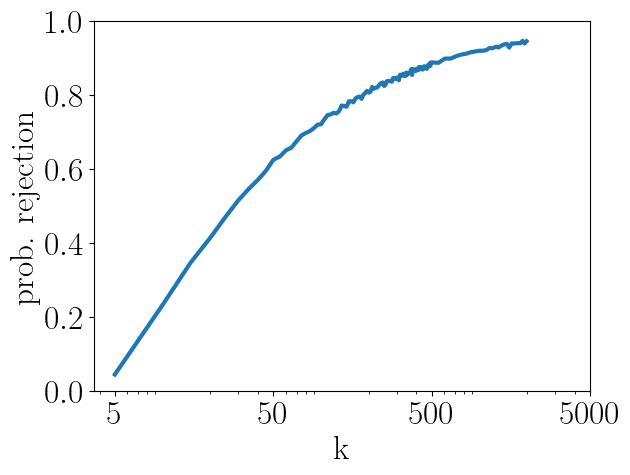
\includegraphics[width=.48\textwidth]{pics/failProbPlotMultinom.png}}
	\caption{Experiments on data generated by a simulation, showing the need for multiple tests correction.
		%
		The data has two protected groups, rankings are created by a multinomial process (``rolling a 3-sided dice'') with $p_G = (0.33, 0.33)$.
		%
		These rankings should have been rejected as unfair at a rate $\alpha = 0.1$.
		%
		However, we see that the rejection probability increases with $k$.
		%
		Note the scale of $k$ is logarithmic.}
	\label{fig:why-adjustment-is-needed-multinomial}
\end{figure}
To illustrate why this correction is needed, observe Figure~\ref{fig:why-adjustment-is-needed-multinomial}, which assumes two protected groups with $p_1=p_2=\frac{1}{3}$.
%
This figure is generated by simulation, generating rankings with the process described above.
%
It shows the probability of those rankings being rejected by our ranked group fairness test with $\alphaadj=0.1$.
%
Generally, we can see that the probability of a Type-I error (declaring this fair ranking as unfair) is higher than $\alpha = 0.1$.
%
Therefore, depending on $k$ we would need to change the value of $\alpha$, if we want to achieve a rejection rate of $0.1$.
%
If the $k$ tests were independent, we could use $\alphaadj = 1 - (1 - \alpha)^{1/k}$ (i.e., {\v S}id{\'a}k's correction), but given the positive dependence, the false negative rate is smaller than the bound given by {\v S}id{\'a}k's correction.

\subsection{General Procedure}
\label{subsec:general-process}
%
With the presence of more than one protected group, the analytical extension of the model adjustment to a multinomial setting is too complex to be written into a closed formula.
%
In contrast to the model adjustment for one protected group which we used in~\cite{zehlike2017fair} (see also Section~\ref{sec:adjustment-binomial}), we found no analytical way to calculate all permutations which pass or fail the test.
%
Therefore we develop an experimental procedure to adjust $ \alpha $:
%
\begin{enumerate}
	\item Get input $ p_G, k, \alpha $.
	\item Build mTree with input $ \alpha $.
	\item Create $M$ rankings by rolling a biased $ |G| $-sided dice with each side's probability to show corresponding to a minimum proportion in vector $ p_G $.
	\item Test all those rankings against the mTree and count how many tests fail.
	%
	Remember that we want to observe a maximum failure probability of $ \failprob=\alpha $, because all rankings created by this multinomial stochastic process are considered to be inherently fair.
	\item If $ \failprob \neq \alpha $, we choose a new $ \alphaadj $ using a binary search heuristic.
	\item Now we build a new mTree using $ \alphaadj $ and repeat the procedure until $ \failprob \approx \alpha $.
\end{enumerate}
%
Once we found $\alphaadj$ we can recompute the mTrees from Figures~\ref{fig:mtree-symmetric-unadjusted} and~\ref{fig:mtree-asymmetric-unadjusted} to obtain an overall significance level of $\alpha = 0.1$.
%
Figures~\ref{fig:mtree-symmetric-adjusted} and~\ref{fig:mtree-asymmetric-adjusted} show the adjusted mTrees with the same parameters $p_G$.
\begin{figure}[h]
	\centering
	\begin{forest}
		for tree={
			child anchor=west,
			parent anchor=east,
			grow'=east,
			draw,
			anchor=west,
		}
		[{[0, 0]}
		[{[0, 0]}
		[{[0, 0]}
		[{[0, 0]} 
		[{[0, 0]}
			[{[1, 0]}
			[{[1, 0]}
				[{[2, 0]}
				[{[2, 0]}
					[{[3, 0]}]
					[{[2, 1]}]
				]]
				[{[1, 1]}, name=doubled1
				[{[1, 1]}
				[{[1, 1]}
				]]]
			]]
			[{[0, 1]}
			[{[0, 1]}, name=parentDoubled1
				[{[0, 2]}
				[{[0, 2]}
					[{[1, 2]}]
					[{[0, 3]}]
				]]
			]]
		]]]]]]
		\draw (parentDoubled1.east)--(doubled1.west);
	\end{forest}
	\CaptionMargin
	\caption{Example of an mTree with two protected groups with minimum proportions $ p_G=[1/3, 1/3] $ and $ \alphaadj=0.1 $. Compared to figure~\ref{fig:mtree-symmetric-unadjusted} this tree is less strict such that its \emph{total} probability $ \alphaadj $ of rejecting a fair ranking (i.e. a type-1-error) is 0.1.
	\label{fig:mtree-symmetric-adjusted}}
	\tablemargin
\end{figure}

\begin{figure}[h]
	\centering
	\begin{forest}
		for tree={
			child anchor=west,
			parent anchor=east,
			grow'=east,
			draw,
			anchor=west,
		}
		[{[0, 0]}
			[{[0, 0]}
				[{[0, 0]}
					[{[1, 0]}
						[{[1, 0]}
							[{[2, 0]}
								[{[2, 1]}
									[{[2, 1]}, name=doubled2, before drawing tree={y-=1em}
										[{[2, 1]}, before drawing tree={y-=1em}
											[{[3, 1]}, before drawing tree={y-=1em}]
											[{[2, 2]}, before drawing tree={y-=1em}]
										]
									]
								]
							]
							[{[1, 1]}, name=doubled1
								[{[1, 1]}, name=parentDoubled2
									[{[1, 2]}, name=doubled3, before drawing tree={y-=1em}
										[{[1, 2]}, before drawing tree={y-=1em}
											[{[1, 2]}, before drawing tree={y-=1em}]
										]
									]
								]
							]
						]]							
					[{[0, 1]}
						[{[0, 1]}, name=parentDoubled1
							[{[0, 2]}
								[{[0, 2]}, name=parentDoubled3
									[{[0, 3]}, before drawing tree={y-=1em}
										[{[0, 3]}, before drawing tree={y-=1em}
											[{[1, 3]}, before drawing tree={y-=1em}]
											[{[0, 4]}, before drawing tree={y-=1em}]
										]
									]
								]
							]
						]]
					]]]
		\draw (parentDoubled1.east)--(doubled1.west);
		\draw (parentDoubled2.east)--(doubled2.west);
		\draw (parentDoubled3.east)--(doubled3.west);
	\end{forest}
	\CaptionMargin
	\caption{Example of an mTree with two protected groups with minimum proportions $ p_G=[0.2, 0.4] $ and a corrected $ \alpha_c=0.1 $. 
	%
	The tree is less strict than the mTree in Figure~\ref{fig:mtree-asymmetric-unadjusted}.
	%
	The adjusted tree yields an overall false-negative rate of $ \alpha_c=0.1 $ when testing rankings for ranked group fairness.
	\label{fig:mtree-asymmetric-adjusted}}
	\tablemargin
\end{figure}

\subsection{Optimizations for MTree Calculation}
\label{subsec:mtree-optimization}
In this subsection we explain how we optimize the adjustment procedure to reduce complexity, as it requires to compute a new mTree at each iteration which is expensive on its own. 
%
Furthermore, depending on the level of accuracy needed, a large number of iterations $M$ might be required and the binary search heuristic may need many steps to find $\alpha$, if large intervals have to be searched.
%
We use three strategies to drastically reduce computational costs of this simulation-based adjustment:
%
\begin{inparaenum}[(i)]
%
\item we reduce the space requirements of the mTree structure;
%
\item we construct the tree level by level and reject if the ranking does not satisfy any node in a level;
%
\item we exploit the monotonicity of $\alphaadj$ with respect to $\alpha$ and use a regression procedure to speed up the binary search.
\end{inparaenum}

\subsubsection{Reducing mTree Space Requirements.} 
We improve the mTree data structure by excluding the calculation and storage of redundant information.
%
First we store each node only once at each level and duplicate nodes are combined into a single node with multiple parents.
%
Furthermore we reduce the size of the mTree by actually leaving out the parent-child relationship and merely storing the nodes itself together with their respective depth levels.
%
Figures~\ref{fig:mtree-symmetric-adjusted} and~\ref{fig:mtree-asymmetric-adjusted} show the mTree structure with all parent-child relations as edges.
%
We leave out these edges, thus reducing space, because we can prove that, if a single node exists on each level, which accepts a given ranking as fair, then a valid path to that node exists in the tree.

Before we can prove this property, we need to introduce the following definition, which formalizes what a successful mTree test at level $i$ looks like.
%
\begin{definition}[Successful mTree Testing]
\label{def:valid-mtree-test}
Let $\tau$ be a ranking of size $k$ and $\tau_{G,i}=(\tau_{1},\ldots,\tau_{|G|})$ the numbers of ranked protected elements from group $1,\ldots,|G|$ up to position $i$.
%
Let furthermore $MT$ be a $mTree$, with $MT_{G,i}=[m_1(i),\ldots,m_{|G|}(i)]$ the number of protected candidates of group $1,\ldots,|G|$ required up to position $i$.
%
We write $\tau_{G,i} \geq m_{G,i}$ if $\tau_g \geq m_g$ for all $g=1,\ldots,|G|$.
%
We call a test on level $i$ of $MT$ successful, iff $\tau_{G,i} \geq m_{G,i}$.
\end{definition}
%
Again, in order to remove the parental relationships in the mTree, thus reducing storage space, we have to prove that, if we test a ranking on each level of the mTree successfully, the entire ranking will be fair according to the ranked group fairness definition.
%
We prove this by showing that, if a ranking passes the test for any two nodes $n_1$ and $n_2$ at two consecutive levels $h$ and $h+1$, and $n_1$ is \emph{not} a parent of $n_2$, then all actual children of $n_1$ will have a weaker requirement than $n_2$ and will hence also test successfully.
%
Furthermore we show that all nodes at level $h+1$ for which the ranking fails the test are part of a path that already rejected it as unfair at level $h$.
%
Consider an example from Figure~\ref{fig:mtree-symmetric-adjusted} : Let us assume a ranking passes the test at level $9$ with exactly the required protected items $[1,1]$.
%
Now lets assume that at level $10$, the given ranking would pass the test for node $[2,1]$, which is not a successor of $[1,1]$.
%
In fact we see that the actual successor of $[1,1]$ is a node with the same configuration $[1,1]$.
%
However, if our ranking passes the test for the stricter node $[2,1]$, it also passes for $[1,1]$ and thus we do not need to know the true parent of $[2,1]$.
%
Note that the ranking would fail at node $[3,0]$, but with $[1,1]$ at level 9 it would have failed already at $[3,0]$'s predecessor $[2,0]$.
%
\begin{theorem}
\label{theorem:lazy-mTree-test}
Let $MT$ be a mTree and $\tau$ a ranking of size $k$.
%
There exists at least one successful test for $\tau$ at each level of $MT$,
iff there exists a valid path from the root of $MT$ to a leaf of $MT$.
\end{theorem}
%
\begin{proof}
	\label{proof:lazy-mTree-test}
	It is clear that at least one successful test per level is necessary for the path to exist.
	%
	Let us proof that one successful test is a sufficient condition for the path to exist.
	%
	Let $MT$ be a mTree and $\tau$ be a ranking that passes the test at level $h$ of $MT$.
	%
	Let $m_{G,h}=[m_{1}(h), \ldots, m_{|G|}(h)]$ be the node on level $h$ that successfully tested $\tau$.
	%
	Let further be $\tau_g(h)$ the number of protected candidates of group $g$ ranked at up to position $h$.
	%
	Without loss of generality let $\sum_{g=1}^{|G|} |m_{g}(h) - \tau_{g}(h)| = 0$, meaning that the ranking includes the exact amount of required protected candidates at level $h$ and not more.
	%
	Let $m_{G,(h+1)}$ be a node which tests $\tau$ successfully on level $h+1$ with $\sum_{g=1}^{|G|} |m_{g}(h+1) - \tau_{g}(h+1)| = 0$.
	%
	For all entries $m_{g}(h+1)$ of $m_{G,(h+1)}$ it is that $m_{g}(h) \leq m_{g}(h+1)$ by construction of the mTree, in which requirements for protected candidates can only increase or stay the same, but cannot decrease.

	\noindent We can now distinguish between the following two cases:
	\\
	\textbf{Case 1:} $m_{G,(h+1)}$ is a child of $m_{G,h}$.
	%
	Then they form a path. %UNNECESSARY:% Note that $\sum_{g=1}^{|G|} (m_{g}(h+1) - m_{g}(h) \leq 1)$.
	\\
	\textbf{Case 2:} $m_{G,(h+1)}$ is not a child of $m_{G,h}$.
	%
	Let now ${m'}_{G,(h+1)}$ be a child of $m_{G,(h)}$.
	%
	Because of $\sum_{g=1}^{|G|} |m_{g}(h) - \tau_{g}(h)| = 0$, and a successful test at level $h+1$, the following inequations hold: $\sum_{g=1}^{|G|} |m_{g}(h) - m_g(h+1)| \leq 1$ and $\sum_{g=1}^{|G|} |m_{g}(h) - m'_g(h+1)| \leq 1$.
	%
	If $\sum_{g=1}^{|G|} |m_{g}(h) - m_g(h+1)| = \sum_{g=1}^{|G|} |m_{g}(h) - m'_g(h+1)| = 0$ or $\sum_{g=1}^{|G|} |m_{g}(h) - m_g(h+1)| = \sum_{g=1}^{|G|} |m_{g}(h) - m'_g(h+1)| = 1$, it follows that $m_{G,(h+1)} = {m'}_{G,(h+1)}$ and we would have a contradiction with the fact that ${m'}_{G,(h+1)}$ is not a child of $m_{G,h}$, because then the nodes would be equal or different by one unit in one position.

	Hence, we need that either
	(2.1) $\sum_{g=1}^{|G|} |m_{g}(h) - m_g(h+1)| = 1$ and $\sum_{g=1}^{|G|} |m_{g}(h) - m'_g(h+1)| = 0$,
	or
	(2.2) $\sum_{g=1}^{|G|} |m_{g}(h) - m_g(h+1)| = 0$ and $\sum_{g=1}^{|G|} |m_{g}(h) - m'_g(h+1)| = 1$.
	%
	Case (2.1) means because of $\sum_{g=1}^{|G|} |m_{g}(h) - m_g(h+1)| = 1 < \sum_{g=1}^{|G|} |m_{g}(h) - m'_g(h+1)| = 0$ that the mTree accepts a ranking with one more protected candidate than required by the actual child of $m_{G,h}$, which contradicts our hypothesis that the ranking included the exact amount of required protected candidates. It follows that if we test $\tau_g (h+1)$ successfully with $m_{G,h+1}$ it would also satisfy ${m'}_{G,h+1}$.
Case (2.2) is impossible according to algorithm \ref{alg:imcdf}.
In detail, if $\sum_{g=1}^{|G|} |m_{g}(h) - m_g(h+1)| = 0$ it means that $ m_g(h+1) = m_{g}(h)$ and therefore, $F(m_{g}(h);h+1,p_G) > \alpha$ (line $4$ of algorithm \ref{alg:imcdf}). But if for the child of $m_{G,h}$, namely ${m'}_{G,h+1}$ it holds that $\sum_{g=1}^{|G|} |m_{g}(h) - m'_g(h+1)| = 1$, it means that
$F(m_{g}(h);h+1,p_G) \leq \alpha$ so that we would have added a new node as a child of $m_{g}(h)$ according to lines  $8-14$ of algorithm \ref{alg:imcdf}. Since both conditions cannot be true at the same time, Case (2.2) can not occur.
\\
In summary, Case (2.1) will only occur if we ranked more protected candidates than needed, and that the resulting test would be more strict than following a path through the mTree.
%
We showed that Case (2.2) is impossible. There is only Case 1 left if we have ranked exactly the number of protected candidates needed at each level of the mTree.
%
It follows that for any ranking that is tested successfully on each level of the mTree, it either was tested by nodes of a path through the mTree or was tested by a series of nodes which is more strict than such path.
\end{proof}
%
\noindent Because of Theorem~\ref{theorem:lazy-mTree-test} we do not need to keep the tree structure (i.e. parental relationship between nodes) and may store only a set of nodes for each level, removing duplicate entries.
%
In case of symmetric minimum proportions $p_G$, we can further save memory and computation time, by reducing mirrored entries such as $[0,2]$ and $[2,0]$.
%
We simply flag a node for which a mirror exists on the same depth level and do not calculate the mirrored branch.

\subsubsection{Adjusting for Small $k$ First}
We use the fact that given a value of $\alpha$, the mTree calculation is not dependent on $ k $, i.e., a mTree for $k=20$ and a mTree for $k=10$ for the same $\alpha$ are equal in the first ten positions.
%
This means that we can start the adjustment from the root node and expand the tree gradually to find the correct $ \alphaadj $, because if $\failprob$ is too high for given $k$, it will also be too high for any $k' > k$. %in particular and we do not have to consider the larger tree, as long as we do not have a good $\alphaadj$ for $k=10$.
%
%In order to show that we can indeed do that, assume that the for loop of algorithm \ref{alg:computeMTree} stops at $k=10$ instead of $k=20$.
%
%Furthermore, we can understand the mTree as a set of rules that a ranking has to satisfy.
%
%If there are no rules for how many protected candidates are required after position $10$, this is equivalent to not requiring more protected candidates after position $10$.
%
%Thus, the probability that a fair ranking is rejected by a shorter mTree is less or equal to a deeper mTree.
%
%We utilize this property to lower computational costs: we calculate the mTree for $k=10$, then create 10000 rankings of length 10 and calculate $ \alphaadj $ under this setting.
%
%Then we set $ k=k+ $\texttt{stepsize}, and repeat the procedure until we reach the desired ranking length.
%
We can see in Figure~\ref{fig:why-adjustment-is-needed-multinomial} that $ \failprob $ grows very fast for small $k$, which makes an early adjustment of $\alpha$ most efficient to save computation time.

%
\begin{figure}[t!]
	\centering
	%
	\subfloat[Training data $R$ for a regression model to predict a good candidate for $\alphaadj$. Each pair $(k_j, \alpha_{c_j})$ is computed for small $k$ using the procedure described in Subsection~\ref{subsec:general-process}. \label{fig:regression-training-data}]
	{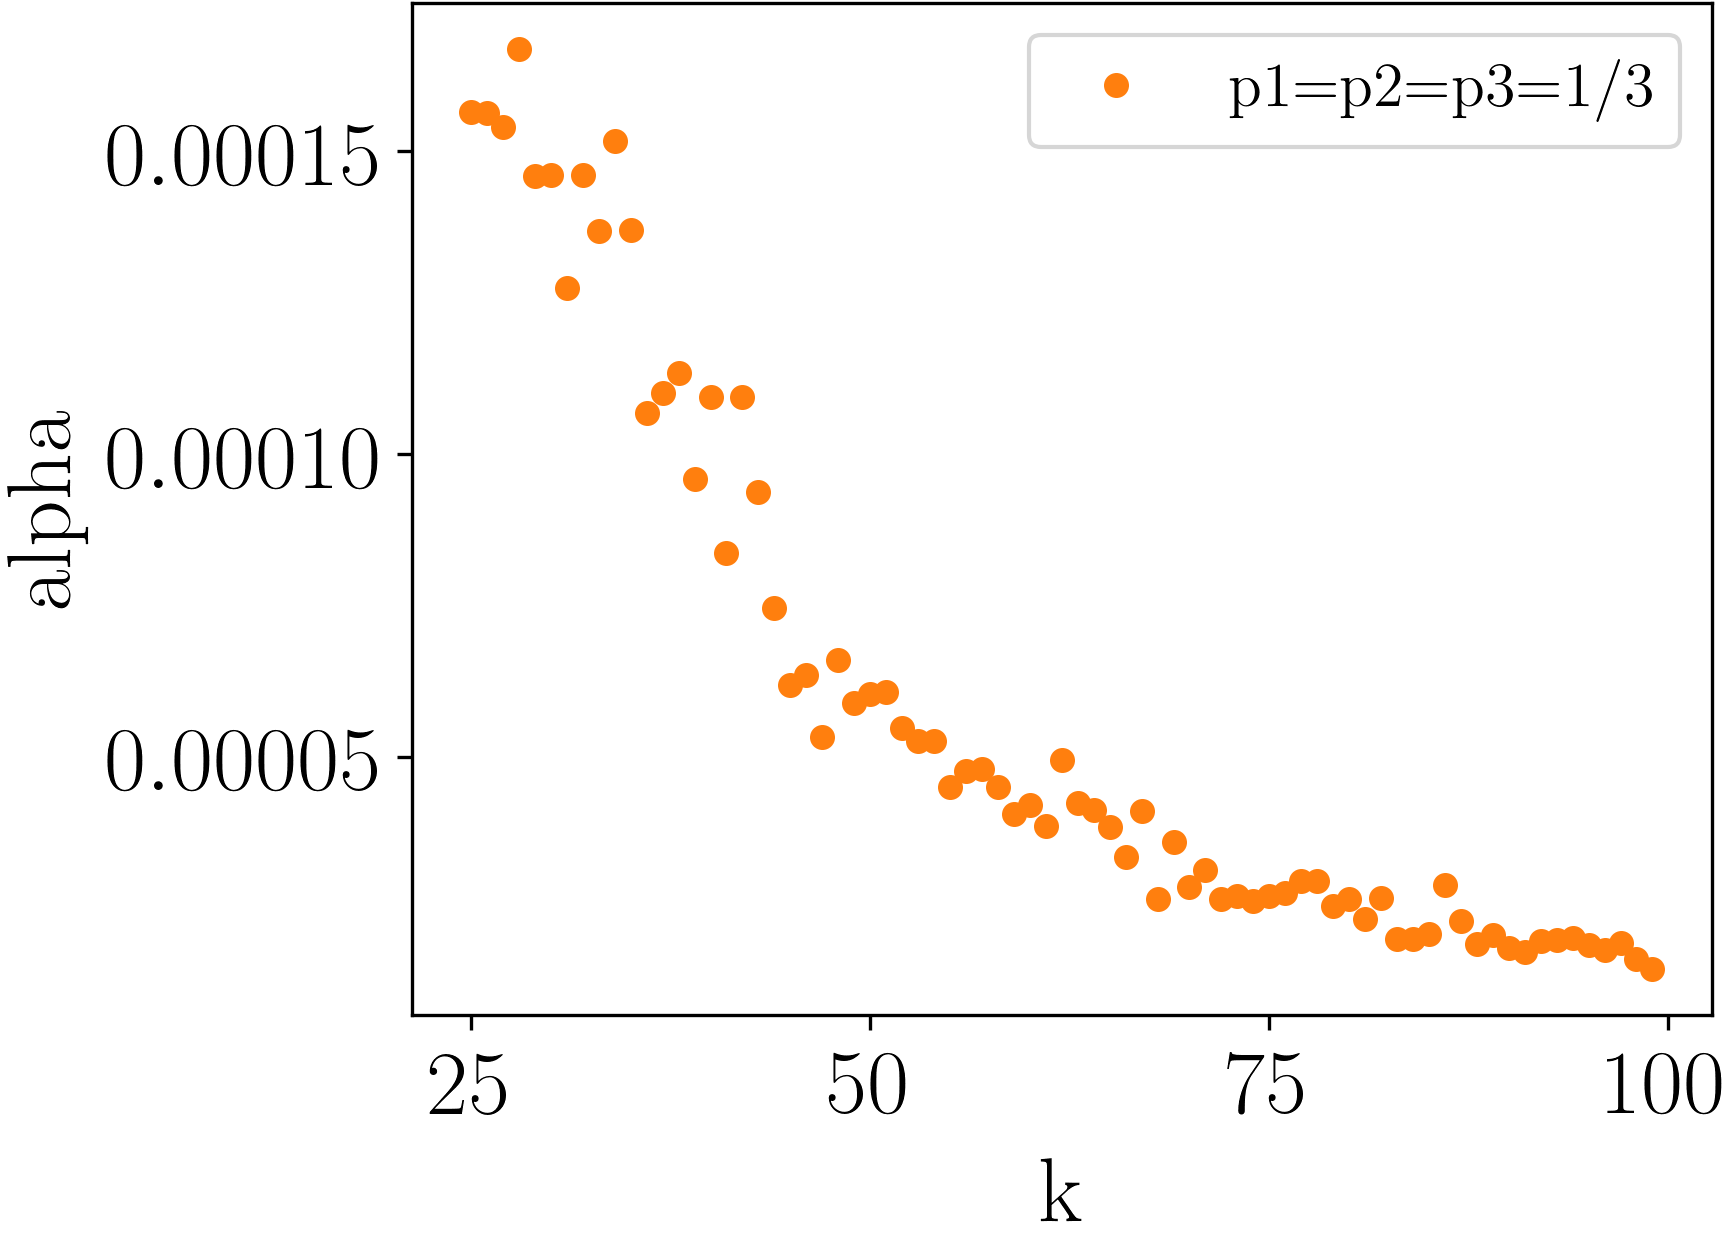
\includegraphics[width=.48\textwidth]{pics/alpha_030303_01.png}}\hfill
	%
	\subfloat[Computation time comparison between binary search only and binary search combined with regression for the multinomial significance adjustment. \inote{"regression" in the figure perhaps could be "regression and binary search"}  \label{fig:regression-time-saved}]
	{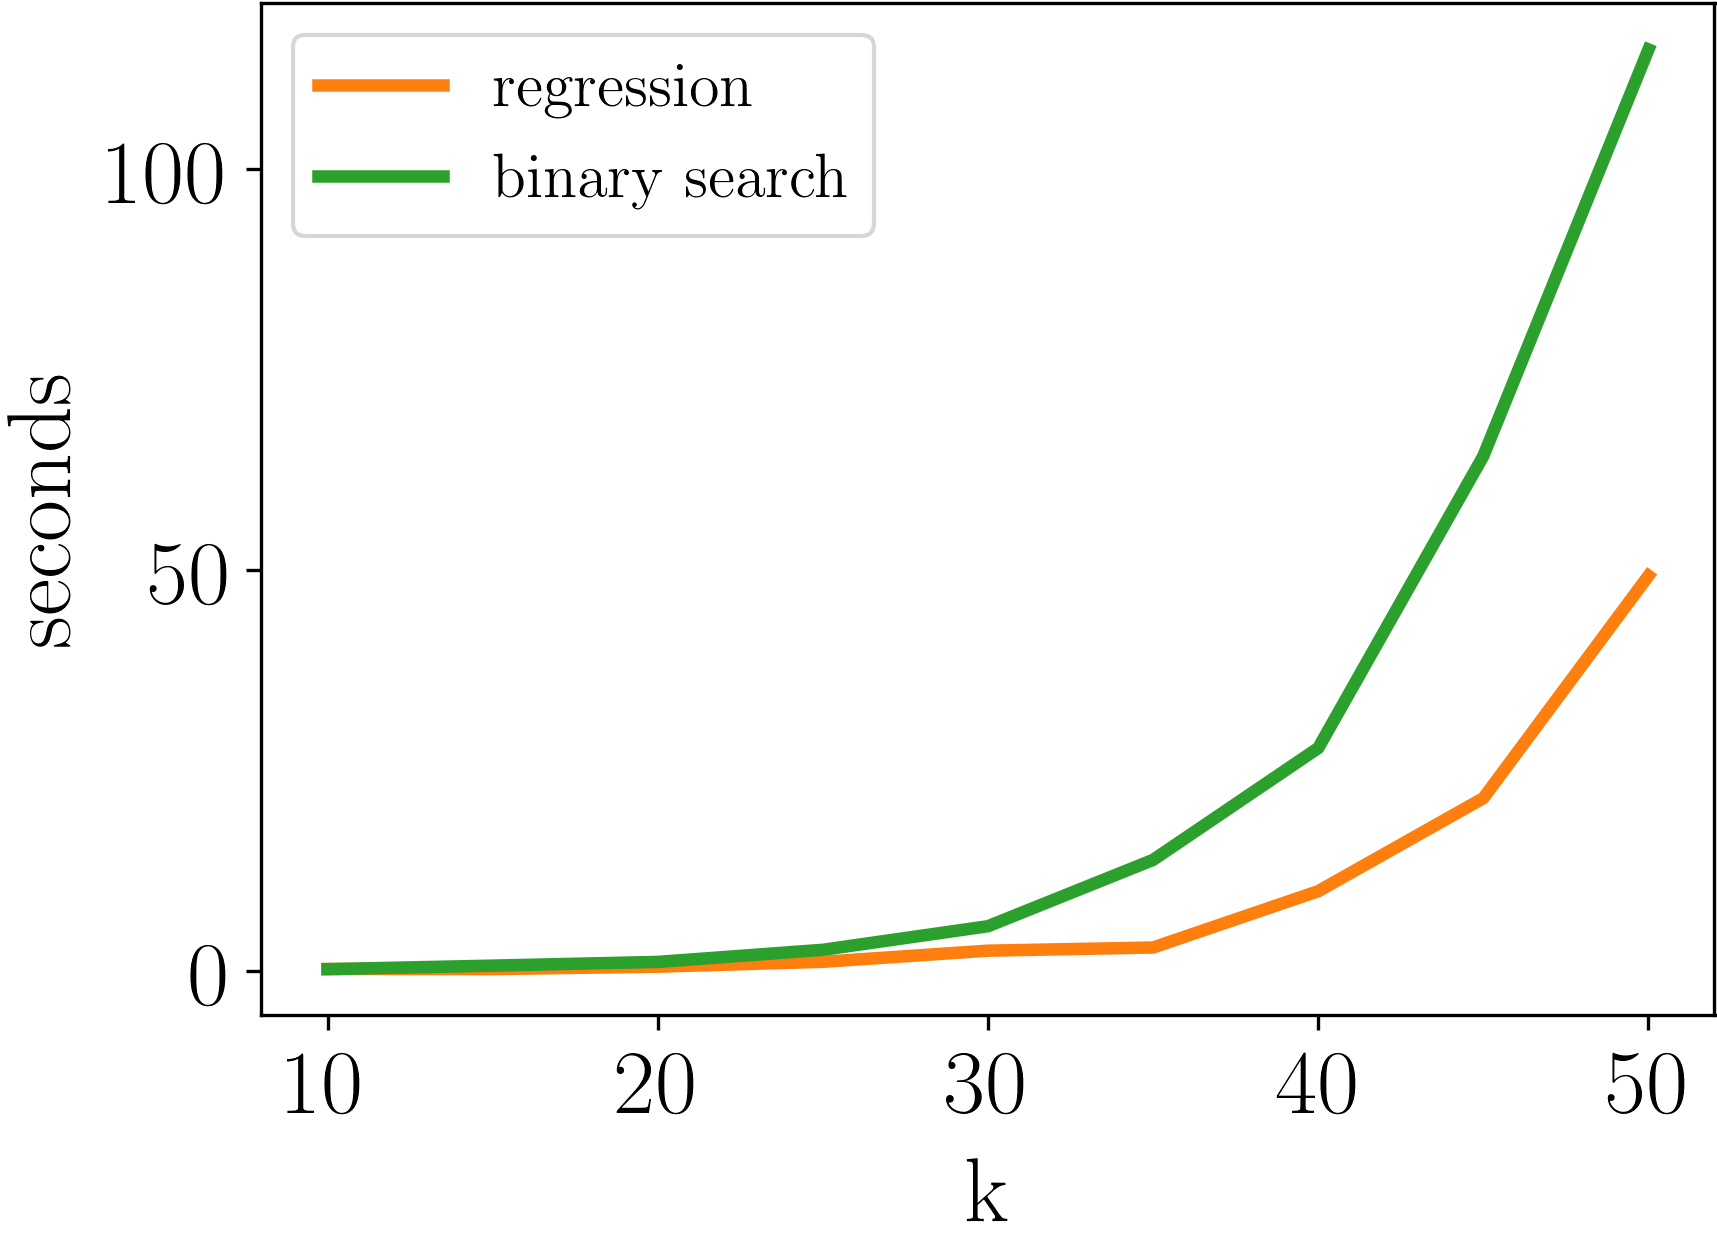
\includegraphics[width=.48\textwidth]{pics/computationTimeRegressionVSBinaryMultinomial.png}}\hfill
	\caption{}
	\label{fig:regression_adjustment_benefits}
	\vspace{-3mm}
\end{figure}
\subsubsection{Finding a Good Starting Candidate for the Binary Search}
We use a second-degree polynomial regression model to get our first estimate for a good $\alphaadj$ candidate and apply the binary search heuristic from that candidate, rather than starting with a random value, that might be very far away from the correct $\alphaadj$.
%
We need a few additional parameters as input: \texttt{kTarget} -- the length of the target ranking, \texttt{kStart} -- the size of the first mTree, \texttt{maxPreAdjustK} -- the maximum size of the mTree before we use regression to predict a good candidate $\alpha_{c_r}$ for the final $\alphaadj$, and \texttt{num\_iterations} -- the number of training instances to be computed.
%
To create a training dataset $R$, we compute \texttt{num\_iterations} small mTrees (i.e. with different $k \leq $ \texttt{maxPreAdjustK}) and adjust the respective $\alpha$ values as described in Subsection~\ref{subsec:general-process}.
%
For each iteration $j$ the pair $(k_j, \alpha_{c_j})$ is stored as a training instance in $R$.
%
Figure~\ref{fig:regression-training-data} shows a training set for $p_G=[1/3, 1/3], \texttt{maxPreAdjustK}=100$.
%
Then a regression model is trained to predict $\alpha_{c_r}$ for \texttt{kTarget}.
%
This $\alpha_{c_r}$ is now used to start the binary search for the correct and final $\alphaadj$.
%
Figure~\ref{fig:regression-time-saved} shows the runtime difference for the model adjustment routine with and without the use of regression.

\subsection{Final Adjustment Algorithm}
Algorithm~\ref{alg:regression_search} shows the overall adjustment algorithm in pseudo-code, which performs the following steps:
%
\begin{enumerate}
	\item Define the necessary parameters: \texttt{kTarget}, \texttt{kStart}, \texttt{maxPreAdjustK}, and \texttt{num\_iterations}
	\item Adjust $\alpha$ for a mTree of size \texttt{kStart} to get $\alpha_{c_1}$ using binary search.
	\item Add pair $\left(\texttt{kStart}, \alpha_{c_1}\right)$ to a regression training set $R$.
	\item \label{stepBegin} Increase $\texttt{kStart}$ by $\texttt{stepsize}=\frac{\texttt{maxPreAdjustK}}{\texttt{num\_iterations}}$
	\item Compute a mTree with parameters $\texttt{kTarget}, p_G, \alpha_{c_1}$ and adjust $\alpha_{c_1}$.
	\item \label{stepEnd} Name result $\alpha_{c_2}$ and add pair $\left(\texttt{kStart}, \alpha_{c_2}\right)$ to $R$.
	\item Repeat steps (\ref{stepBegin}) -- (\ref{stepEnd}) until $\texttt{kStart} == \texttt{maxPreAdjustK}$.
	\item Train a regression model with training data $R$ to predict $\alpha_{c_r}$ for $\texttt{kTarget}$.
	\item Use binary search (Algorithm~\ref{alg:mult_binary}) to find $\alphaadj$ for parameters $k,p_G, \alpha_{c_r}$.
\end{enumerate}
%
\begin{algorithm}[b!]
	\caption{Algorithm \algoReg estimates the corrected significance level $\alphaadj$ such that the mTree $m(\alphaadj , k, p_G)$ has the probability of rejecting a fair ranking $\alpha$}
	\label{alg:regression_search} % But whenever possible refer to this algo. by name not number
	\small
	\AlgInput{\texttt{kStart} -- depth of the mTree to start with; $k$ -- the length of the ranking; $p_G$ -- the desired proportions of the protected groups; $\alpha$ -- the desired significance level;  \texttt{maxPreAdjustK} the maximum depth of the mTrees that are used as training data; \texttt{num\_iterations} -- the number of steps between \texttt{kStart} and \texttt{maxPreAdjustK}}
	\AlgOutput{$\alphaadj$ -- the adjusted significance}
	$R \leftarrow \lbrace \rbrace; \alpha_{\textit{new}} \leftarrow \alpha$	\\
	\AlgComment{divide the interval [$\text{kStart}, \text{maxPreAdjustK}$] into num\_iterations parts}
	$\texttt{stepsize} \leftarrow \max(\frac{\texttt{maxPreAdjustK}}{\texttt{num\_iterations}}, 1)$ \\
	\For{$i\leftarrow 0$ to $\texttt{num\_iterations}$}{
		\AlgComment{adjust $\alpha_{\text{new}}$ for the current kStart}
    	$\alpha_{\text{new}} \leftarrow \textsc{MultinomialBinarySearchAdjustment}(\alpha_{\textit{new}}, \texttt{kStart}, p_G)$ \\
    	\AlgComment{add the pair (kStart, $\alpha_{\textit{new}}$) to the training data $R$}
    	$R.\textit{put}(\texttt{kStart},\alpha_{\textit{new}})$ \\
    	\If{$\texttt{kStart} + \texttt{stepsize} \leq \texttt{maxPreAdjustK}$}{
    		$\texttt{kStart} \leftarrow \texttt{kStart} + \texttt{stepsize}$ \\
    	}\Else{
			break
    	}
    }
    $\texttt{coeffs} \leftarrow R.\textit{train}()$ \AlgComment{returns the vector of predicted coefficients for the curve over $R$}
    $\alpha_{c_r} \leftarrow \texttt{coeffs[0]} + \texttt{coeffs[1]} * k + \texttt{coeffs[2]} * k^2$ \\
    $\alphaadj \leftarrow \textsc{MultinomialBinarySearchAdjustment}(\alpha_{c_r},k,p_G)$ \\
    \Return{$\alphaadj$}
\end{algorithm}

\FloatBarrier
